% ju 08-Jun-22
\documentclass[a4paper,12pt,fleqn,parskip=half]{scrartcl}
\usepackage[ngerman]{babel}
\usepackage[utf8]{inputenc}
\usepackage[T1]{fontenc}

% Schrift
%\usepackage{lmodern}
\usepackage[osf,sc]{mathpazo} 
\usepackage[scale=.9,semibold]{sourcecodepro}   
\usepackage[osf]{sourcesanspro}  

\usepackage[headsepline]{scrlayer-scrpage}
\pagestyle{scrheadings}
\clearpairofpagestyles

\usepackage[table,dvipsnames,usenames]{xcolor}
\usepackage{textcase}
\usepackage{nameref}
\usepackage{hyperref}
\usepackage{tabularx}
\usepackage{multirow}
\usepackage{multicol}
\usepackage{caption, booktabs}
\usepackage{graphicx} 
\usepackage{scrhack}    
\usepackage{url}%% Links
\usepackage[inline]{enumitem}
\usepackage{pifont}
\usepackage{eurosym}% \euro 20,-
\usepackage{amsmath}
\usepackage{amsfonts}
\usepackage{amssymb}
\usepackage{array}            % Extending the array and tabular environments
\usepackage{chngcntr}         % Change the resetting of counters
\usepackage[version=4]{mhchem}
\usepackage{stmaryrd}
\usepackage{siunitx}
\usepackage{float}
\usepackage{csquotes}
\usepackage{subcaption}
\usepackage{mathtools}
\usepackage{icomma}%Dezimaltrennzeichen
\usepackage{multimedia}%Video: \movie[externalviewer]{(video.mov)}{video.mov}
\usepackage{epstopdf}
\usepackage{footnote}
\usepackage{qrcode}% Anwendung: \qrcode[hyperlink,level=Q,version=2,height=1cm]{\website}
\usepackage{underscore}% Unterstrich ____

% PDF Dokumente einbinden
\usepackage{pdfpages}% \includepdf[pages=-]{Tabellen/Excel.pdf}
\RequirePackage{lastpage}  % Pagecounter

\addto\captionsngerman{%
\renewcommand{\figurename}{Abb.}
\renewcommand{\tablename}{Tab.}
}

% listings
\usepackage{listings}
\lstset{basicstyle=\linespread{1}\ttfamily\small,floatplacement=!htb,captionpos=t,abovecaptionskip=.5\baselineskip,belowcaptionskip=.5\baselineskip,upquote=true,showstringspaces=false,inputencoding=utf8,tabsize=4,
    	keywordstyle=\bfseries ,
	commentstyle=\color{rot5},
	stringstyle=\color{orange},
	breaklines=true,
  	postbreak=\mbox{\textcolor{black}{$\hookrightarrow$}\space},
	breakatwhitespace=false
}
\lstset{literate={á}{{\'a}}1 {é}{{\'e}}1 {í}{{\'i}}1 {ó}{{\'o}}1 {ú}{{\'u}}1 {Á}{{\'A}}1 {É}{{\'E}}1 {Í}{{\'I}}1 {Ó}{{\'O}}1 {Ú}{{\'U}}1 {à}{{\`a}}1 {è}{{\`e}}1 {ì}{{\`i}}1 {ò}{{\`o}}1 {ù}{{\`u}}1 {À}{{\`A}}1 {È}{{\'E}}1 {Ì}{{\`I}}1 {Ò}{{\`O}}1 {Ù}{{\`U}}1 {ä}{{\"a}}1 {ë}{{\"e}}1 {ï}{{\"i}}1 {ö}{{\"o}}1 {ü}{{\"u}}1 {Ä}{{\"A}}1 {Ë}{{\"E}}1 {Ï}{{\"I}}1 {Ö}{{\"O}}1 {Ü}{{\"U}}1 {â}{{\^a}}1 {ê}{{\^e}}1 {î}{{\^i}}1 {ô}{{\^o}}1 {û}{{\^u}}1 {Â}{{\^A}}1 {Ê}{{\^E}}1 {Î}{{\^I}}1 {Ô}{{\^O}}1 {Û}{{\^U}}1 {œ}{{\oe}}1 {Œ}{{\OE}}1 {æ}{{\ae}}1 {Æ}{{\AE}}1 {ß}{{\ss}}1 {ű}{{\H{u}}}1 {Ű}{{\H{U}}}1 {ő}{{\H{o}}}1 {Ő}{{\H{O}}}1 {ç}{{\c c}}1 {Ç}{{\c C}}1 {ø}{{\o}}1 {å}{{\r a}}1 {Å}{{\r A}}1 {€}{{\EUR}}1 {£}{{\pounds}}1 {~}{{\textasciitilde}}1 {-}{{-}}1 }

% bibliography
\usepackage[
    bibencoding=utf8,
    backend=biber,% bibtex, biber
    backref=false,backrefstyle=three+,url=true,urldate=comp,abbreviate=false,maxnames=20
]{biblatex} %Paket laden
\DeclareBibliographyCategory{cited}
\let\defaultcite\cite\renewcommand*\cite[2][]{\addtocategory{cited}{#2}\defaultcite[#1]{#2}}
\let\defaulttextcite\textcite\renewcommand*\textcite[2][]{\addtocategory{cited}{#2}\defaulttextcite[#1]{#2}}
\setcounter{biburllcpenalty}{7000}
\setcounter{biburlucpenalty}{8000}
\AfterPackage{biblatex}{
	\PreventPackageFromLoading[\errmessage{Sie haben versucht, das Cite-Paket zu laden, das nicht mit biblatex kompatibel ist.}]{cite}
}

\hypersetup{%
	%pdftitle={\titel},
	%pdfsubject={Latex},
	%pdfauthor={\autor},
	%pdfcreator={\autor}, 
	bookmarksnumbered=true,
	breaklinks=true,
	%colorlinks=true,	   
	linkcolor=rot5,		
	filecolor=blau5,		
	urlcolor=blau5,			
	citecolor=ForestGreen
}

\linespread{1.1}
\setlist{itemsep=0pt}
\widowpenalty10000
\clubpenalty10000
\tolerance1000   

\usepackage[left=2cm,right=2cm,top=1cm,bottom=1cm,includeheadfoot]{geometry}
%\usepackage[left=4cm,right=2cm,top=1cm, bottom=1cm,includeheadfoot]{geometry}
%\usepackage[left=6cm,right=1cm,top=1cm, bottom=1cm,includeheadfoot]{geometry}
%\usepackage[landscape=true,left=2cm,right=2cm,top=1cm,bottom=1cm,includeheadfoot]{geometry}%quer

% eigene Farbe definieren
% Adobe Prozessfarben: CMYK: 100,50,0,35 -> 1,0.5,0,0.35
\definecolor{orange}{cmyk}{0,0.55,0.61,0}   % 0,55,61,0
\definecolor{blau5}{cmyk}{1,0.77,0.1,0.01}  % 100,77,10,
\definecolor{rot5}{cmyk}{0.22,1,1,0.19}     % 22,100,100,19
\definecolor{grau2}{cmyk}{0,0,0,0.1}        % 0,0,0,40
\definecolor{blau}{cmyk}{0.93,0.66,0,0.21}% 

% Literatur
\bibliography{content/literatur}
\bibliography{content/literatur-kfz}
\bibliography{content/literatur-sport}

%%%%%%%%%%%%%%%%%%%%%%%%%%%%%%%%%%%%%%%%%%%%%%%%%%%%%%%
\newcommand{\name}{Jan Unger}
\newcommand{\thema}{Gemischbildung-Ottomotor}
\newcommand{\quelle}{\name}
\newcommand{\website}{https://bw-ju.de/}
\newcommand{\github}{https://github.com/ju1-eu}
%%%%%%%%%%%%%%%%%%%%%%%%%%%%%%%%%%%%%%%%%%%%%%%%%%%%%%%

\ihead{\textbf{Quelle:} \quelle}%{Kopfzeile innen}
\ohead{\textbf{Datum:} \today}  %{Kopfzeile außen}
\ifoot{\textbf{Thema:} \thema}  %{Fußzeile  innen}
\ofoot{Seite {\thepage} von {\pageref{LastPage}}}%{Fußzeile  außen}

\title{\thema}
\author{\name}
\date{\today}

\begin{document}
	%%%%%%%%%%%%%%%%%%%%%%%%%%%%%%%%%%%%%%%%%%%%%%%%%%%%%%%%%%%%%%%%%%
	\begin{abstract}
		\center
		\textbf{\Large \thema}%14pt
		
		\vspace{1.5em}
		%\datum	
		%\qrcode[hyperlink,level=Q,version=2,height=1cm]{\website}
		\qrcode[hyperlink,level=Q,version=2,height=1cm]{\github}
		
		\vspace{1.5em} 
		\raggedright
		\textbf{\large Keywords}
		% Checkliste
		\begin{itemize}[label=\checkmark]
			\item Begriff
		\end{itemize}
	\end{abstract}
    %%%%%%%%%%%%%%%%%%%%%%%%%%%%%%%%%%%%%%%%%%%%%%%%%%%%%%%%%%%%%%%%%%

	% anpassen
	%\input{content/tex/neu}
	%ju 08-Jun-22 Gemischbildung-Ottomotor.tex
\section{Gemischbildungssysteme}\label{gemischbildungssysteme}

sollen für jeden Betriebszustand des Motors ein Kraftstoff-Luft-Gemisch
herstellen, das in der \emph{Menge ausreichend} ist und im Motor
möglichst \emph{vollständig verbrannt} wird.

\section{Betriebszustände}\label{betriebszustaende}

\begin{itemize}
\item
  \textbf{Kaltstart}

  \begin{itemize}
  \item
    Kraftstoff kondensiert an kalten Saugrohr- und Zylinderwänden
  \item
    $\to$ sehr fettes Gemisch (bis $\lambda = 0,3$) nötig
  \end{itemize}
\item
  \textbf{Warmlauf}

  \begin{itemize}
  \item
    Kondensationsverluste verringert sich
  \item
    $\to$ Kraftstoffmenge wird temperaturabhängig verringert
  \end{itemize}
\item
  \textbf{Leerlauf}
\item
  \textbf{Übergang, Beschleunigung}

  \begin{itemize}
  \item
    beim Öffnen der Drosselklappe magert das Gemisch kurzzeitig ab
  \item
    $\to$ kurzzeitig mehr Kraftstoff einspritzen
  \end{itemize}
\item
  \textbf{Teillast}
\item
  \textbf{Volllast}

  \begin{itemize}
  \item
    maximale Motorleistung bei voll geöffneter Drosselklappe
  \item
    $\to$ Anreicherung des Gemisches auf $\lambda = 0,85 \dots 0,95$
  \end{itemize}
\item
  \textbf{Schubabschaltung}

  \begin{itemize}
  \item
    Drosselklappe geschlossen bei hoher Drehzahl (Bergab fahren oder Fuß
    vom Gas bei hoher Geschwindigkeit)
  \item
    $\to$ keine Einspritzung von Benzin bis Drosselklappe wieder
    geöffnet
  \end{itemize}
\end{itemize}

\section{Mischungsverhältnis}\label{mischungsverhaeltnis}

beschreibt die \emph{Zusammensetzung des Kraftstoff-Luft-Gemisches}. Man
unterscheidet ein theoretisches und ein praktisches Mischungsverhältnis.

\begin{enumerate}
\item
  \textbf{Theoretisches Mischungsverhältnis} (stöchiometrisches
  Verhältnis):

  \begin{itemize}
  \item
    zur \emph{vollständigen Verbrennung} von $1~kg$ Super werden
    $14,7~Kg$ Luft benötigt
  \end{itemize}
\item
  \textbf{Praktisches Mischungsverhältnis}

  \begin{itemize}
  \item
    weicht je nach Betriebszustand vom theoretischen Verhältnis ab
  \item
    \emph{Fettes Gemisch} (Luftmangel): z. B. $1:13$
  \item
    \emph{Mageres Gemisch} (Luftüberschuss): z. B. $1:16$
  \end{itemize}
\end{enumerate}

\section{Luftverhältnis}\label{luftverhaeltnis}

$\lambda$ ist das Verhältnis zwischen der tatsächlich der Verbrennung
zugeführten Luftmasse und der zur vollständigen Verbrennung theoretisch
erforderlichen Luftmasse

\begin{itemize}
\item
  Luftverhältnis
  $\lambda = \frac{\text{zugeführte Luftmasse in [kg]}} {\text{theoretische Luftmasse in [kg]}}$
\item
  Beim theoretischen Mischungsverhältnis $1:14,7$ ist $\lambda = 1$
\item
  $\lambda = \frac{16~kg}{14,7~kg} > 1$ (mager)
\end{itemize}

\textbf{Mischungsverhältnisse für Super}

\begin{figure}[!ht]% hier: !ht
\centering
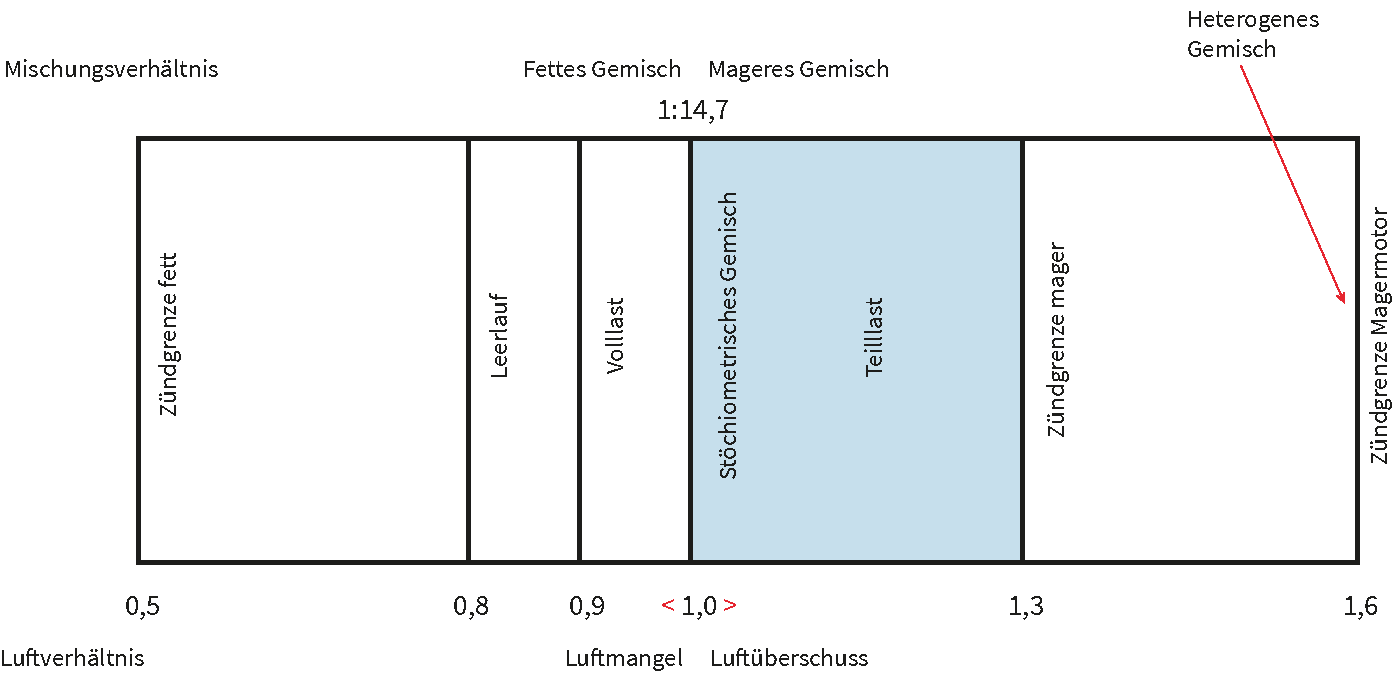
\includegraphics[width=0.6\textwidth]{images/skizze/Mischungs-Luftverhaeltnis.pdf}
\caption{Mischungsverhältnis}
%\label{fig:}%% anpassen
\end{figure}

\section{Gemischzusammensetzung}\label{gemischzusammensetzung}

\begin{enumerate}
\item
  \textbf{Homogenes Gemisch}

  \begin{itemize}
  \item
    im gesamten Brennraum ist die Gemischzusammensetzung gleich
  \item
    Einspritzung im Ansaugtakt
  \item
    braucht Zeit für eine gleichmäßige Durchmischung des
    Kraftstoff-Luft-Gemisches
  \end{itemize}
\item
  \textbf{Heterogenes Gemisch}

  \begin{itemize}
  \item
    im Brennraum gibt es Bereiche unterschiedlicher
    Gemischzusammensetzung (\textbf{Schichtladung})

    \begin{itemize}
    \item
      Fettes Gemisch in der Nähe der Zündkerze ($\lambda = 1$)
    \item
      Mageres Gemisch im äußeren Bereich ($\lambda > 1,3$)
    \item
      späte Einspritzung während des Verdichtungstaktes
    \end{itemize}
  \item
    Saugrohrklappe geschlossen
  \item
    man kann sehr mager fahren, um Sprit zu sparen
  \end{itemize}
\end{enumerate}

\textbf{Ort der Gemischbildung}

\begin{enumerate}
\item
  \textbf{Äußere Gemischbildung} Kraftstoff wird in das Saugrohr
  eingespritzt

  \begin{itemize}
  \item
    Homogenes Gemisch
  \end{itemize}
\item
  \textbf{Innere Gemischbildung} Kraftstoff wird direkt in den Brennraum
  eingespritzt

  \begin{itemize}
  \item
    Heterogenes Gemisch

    \begin{itemize}
    \item
      späte Einspritzung während des Verdichtungstaktes kurz vor Zündung
    \item
      Kraftstoff und Luft kann sich nicht gleichmäßig vermischen
    \end{itemize}
  \item
    Homogenes Gemisch

    \begin{itemize}
    \item
      Einspritzung zu Beginn des Ansaugtaktes
    \end{itemize}
  \end{itemize}
\item
  \textbf{Kombi aus äußere und innere Gemischbildung}
\end{enumerate}

\section{Leistungsregelung}\label{leistungsregelung}

\begin{enumerate}
\item
  \textbf{Quantitätsregelung} Motoren mit äußerer Gemischbildung und
  homogenem Gemisch

  \begin{itemize}
  \item
    Je nach Lastzustand ändert sich die Drosselklappe und damit die
    angesaugte Luftmenge.
  \item
    Die Zusammensetzung des Gemisches muss dabei nahezu gleich bleiben
    ($\lambda = 1$)
  \end{itemize}
\item
  \textbf{Qualitätsregelung} Motoren mit innerer Gemischbildung und
  heterogenem Gemisch

  \begin{itemize}
  \item
    Bei geöffneter Drosselklappe wird verschieden viel Kraftstoff
    eingespritzt. Die angesaugte Luftmenge bleibt dabei nahezu gleich
  \item
    Die Zusammensetzung des Gemisches im Brennraum ändert sich somit je
    nach Lastzustand.
  \end{itemize}
\end{enumerate}

\section{Arten der
Benzineinspritzung}\label{arten-der-benzineinspritzung}

\textbf{Vergaser}

Luft wird angesaugt vom Motor, vor der Drosselklappe gibt es eine
Verengung, durch die Verengung erhöht sich die Strömungsgeschwindigkeit
der angesaugten Luft (Venturi-Rohr). Der Kraftstoff im Vergaser gelangt
über eine Düse in Tropfenform in das Ansaugluftgemisch. Durch die hohe
Strömungsgeschwindigkeit der angesaugten Luft wird der Kraftstoff
mitgerissen.

Vorzerstäubung, Feinzerstäubung $\to$ Kraftstoff-Luft-Gemisch

Die Luftdurchflussmenge wird über Luftdruck (Luftdichte) und Temperatur
gemessen. Daraus wird die Düsengröße berechnet und damit die
Kraftstoffmenge.

\textbf{Indirekte Einspritzung}

\emph{Einzelpunkteinspritzung}

\begin{itemize}
\item
  vor der Drosselklappe befindet sich ein Einspritzventil
\item
  die angesaugte Luft wird mit Kraftstoff versetzt, sodass ich hier ein
  Gemisch gebildet habe
\item
  Gemischzusammensetzung war nicht so genau, durch unterschiedliche
  Ansaugwege
\end{itemize}

\begin{table}[!ht]% hier: !ht 
\centering 
	\caption{}% \label{tab:}%% anpassen 
\begin{tabular}{@{}ll@{}}
\hline
\textbf{\#} & \textbf{Beschreibung} \\
\hline
Art der Einspritzung & \textbf{SPI = Single Point Injection} \\
Ort der Einspritzung & Indirekt - vor der Drosselklappe \\
Gemischzusammensetzung & homogen \\
\hline
\end{tabular} 
\end{table}

\emph{Mehrpunkteinspritzung}

\begin{itemize}
\item
  die angesaugte Luft strömt durch die Drosselklappe in das
  Verteilerrohr
\item
  Kraftstoffverteilerrohr mit einzelne Einspitzventilen, die direkt in
  das Saugrohr einspritzen
\item
  Gemischzusammensetzung ist gleich (gleiche Ansaugwege)
\end{itemize}

\begin{table}[!ht]% hier: !ht 
\centering 
	\caption{}% \label{tab:}%% anpassen 
\begin{tabular}{@{}ll@{}}
\hline
\textbf{\#} & \textbf{Beschreibung} \\
\hline
Art der Einspritzung & \textbf{MPI = Multi Point Injection} \\
Ort der Einspritzung & Indirekt - vor das Einlassventil \\
Gemischzusammensetzung & homogen \\
\hline
\end{tabular} 
\end{table}

\textbf{Direkte Einspritzung}

\begin{table}[!ht]% hier: !ht 
\centering 
	\caption{}% \label{tab:}%% anpassen 
\begin{tabular}{@{}ll@{}}
\hline
\textbf{\#} & \textbf{Beschreibung} \\
\hline
Art der Einspritzung & \textbf{MPI = Multi Point Injection} \\
Ort der Einspritzung & Direkt - in den Zylinder \\
Gemischzusammensetzung & homogen oder heterogen \\
\hline
\end{tabular} 
\end{table}

\section{Öffnung der
Einspritzventile}\label{oeffnung-der-einspritzventile}

\begin{itemize}
\item
  Simultane Einspritzung
\item
  Sequenzielle Einspritzung
\item
  Zylinderselektive Einspritzung
\end{itemize}

\section{Zündanlage}\label{zuendanlage}

\textbf{Zündanlage mit Unterbrecherkontakt}

Bat. 12 V $\to$ Zündspannung 40.000 V

Batterie - 30 - Zündschalter - 15 - Zündspule

\begin{itemize}
\item
  1 - Unterbrecherkontakt - Masse wird geschaltet durch Nocken

  \begin{itemize}
  \item
    geschlossen - in Primärspule baut sich Magnetfeld auf
  \item
    offen - Magnetfeld bricht zusammen, es wird eine Spannung in der
    Sekundärspule indiziert - Spannung geht weiter an den Zündverteiler
  \end{itemize}
\item
  4 - Zündverteiler - Zündkerze - Zündfunken - Masse
\end{itemize}

\textbf{Zündanlage mit Einzelfunkzündspule}

\begin{itemize}
\item
  Eingabe - Wann soll gezündet werden?

  \begin{itemize}
  \item
    Positionsgeber an Nockenwelle und Fahrpedal
  \end{itemize}
\item
  Verarbeitung erfolgt im Steuergerät

  \begin{itemize}
  \item
    Kennfeld - abhängig von Drehzahl und Last wird ein Zündwinkel
    berechnet
  \end{itemize}
\item
  Ausgabe an Zündspule
\end{itemize}

\section{Sensoren und Aktoren}\label{sensoren-und-aktoren}

\begin{table}[!ht]% hier: !ht 
\centering 
	\caption{}% \label{tab:}%% anpassen 
\begin{tabular}{@{}lll@{}}
\hline
\textbf{\#} & \textbf{Sensoren} & \textbf{Aktoren} \\
\hline
\textbf{Zentraleinspritzung} & Drehzahlgeber &
Drosselklappenansteller \\
& Motortemperaturfühler & Regenerierventil \\
& Lufttemperaturfühler & Einspritzventil \\
& Drosselklappenpotentiometer & \\
& Lambdasonde & \\
& OT-Geber & \\
\textbf{MED - Motronic} & Luftmassenmesser & Kraftstoffpumpe \\
& Saugrohrdrucksensor & E-Gas Stellmotor \\
& Differenzdrucksensor & Lambdasondenheizung \\
& Fahrpedalsensor & NOx-Sensorheizung \\
& NOx-Sensor & Tankentlüftungsventil \\
& Abgastemperatursensor & Abgasrückführventil \\
& Saugrohrklappenpotentiometer & Kraftstoffdruckregelventil \\
& & Saugrohrklappenventil \\
\hline
\end{tabular} 
\end{table}


	%%%%%%%%%%%%%%%%%%%%%%%%%%%%%%%%%%%%%%%%%%%%%%%%%%%%%%%%%%%%%%%%%%
    % Bibliographie
    \printbibliography[category=cited]
\end{document}
